\documentclass[11pt]{article}
\usepackage[margin=0.78in]{geometry}
\usepackage{booktabs}
\usepackage{graphicx}
\usepackage{amsmath}
\usepackage{xcolor}
\usepackage[hidelinks]{hyperref}
\usepackage{microtype}
\usepackage{float}
\setlength{\parindent}{0pt}
\setlength{\parskip}{5pt}
\newcommand{\verdict}[1]{\fcolorbox{black}{gray!10}{\strut\texttt{#1}}}
\title{Native-VC Brill Collapse:\\Outer-Boundary Convergence and N256 KO Scan}
\author{AthenaK numerical investigation}
\date{24 August 2026}
\begin{document}
\maketitle

\begin{abstract}
We isolate two hypotheses in the repaired vertex-centered Cartoon Z4c Brill
calculation. First, production-matched radial constraint inventories and a new
$R_{\rm out}=128M$ common-tree experiment show that the apparent N256--N512
flattening in the old global Figure-2 norms is an outer-boundary/shell effect.
Second, an independent $R_{\rm out}=16M$ N256 scan shows that stronger
Kreiss--Oliger (KO) dissipation strongly delays the late refinement cascade.
The two conclusions are kept separate; no production default is changed.
\end{abstract}

\section{Scope and numerical authority}

All work starts from commit
\texttt{953f2724c00a2efd2f9fad91ae9a784639954a3b}.
The production VC transfer, Z4c equations, Cartoon regularization, gauge,
constraint damping, and admissibility gates are unchanged. The boundary
experiment changes only domain size, minimum SMR structure, and absolute level
ceilings. The KO experiment changes only \texttt{z4c/diss}.

The Cartoon history diagnostic already uses
\[
 dV=2\pi\rho\,\sqrt{\det\gamma}\,d\rho\,dz
\]
with canonical native-VC trapezoid ownership. There is no fictitious
collapsed-$y$ width. The reported quantities are extensive squared-constraint
inventories, not square-root norms or RMS values.

\section{Part I: boundary and convergence}

\subsection{Small-domain localization}

At the common terminal time $\tau_c=3.98614742555601M$, the old full-domain
fine-pair orders collapse, while the causally protected interior remains
high-order. The terminal full-square values are:

\begin{table}[H]\centering\small
\begin{tabular}{lrrrrr}
\toprule
 & N128 & N256 & N512 & $p_{128,256}$ & $p_{256,512}$\\
\midrule
C & $5.5801{\times}10^{-2}$ & $3.2813{\times}10^{-3}$ & $1.8063{\times}10^{-3}$ & 4.088 & 0.861\\
H & $2.1558{\times}10^{-2}$ & $3.5049{\times}10^{-4}$ & $1.2550{\times}10^{-4}$ & 5.943 & 1.482\\
M & $8.6428{\times}10^{-3}$ & $4.2832{\times}10^{-4}$ & $5.7349{\times}10^{-5}$ & 4.335 & 2.901\\
Z & $4.0712{\times}10^{-3}$ & $5.0507{\times}10^{-4}$ & $4.0069{\times}10^{-4}$ & 3.011 & 0.334\\
\bottomrule
\end{tabular}
\caption{$R_{\rm out}=16M$ full-domain squared-constraint inventories.}
\end{table}

Inside $r\le4M$, the corresponding $p_{256,512}$ values are 7.831, 7.830,
7.796, and 7.888. For N512, 99.87\% of the old Z inventory is outside
$r=12M$: 50.53\% in $12<r\le16M$ and 49.34\% in the square corners with
$r>16M$.

\begin{figure}[H]\centering
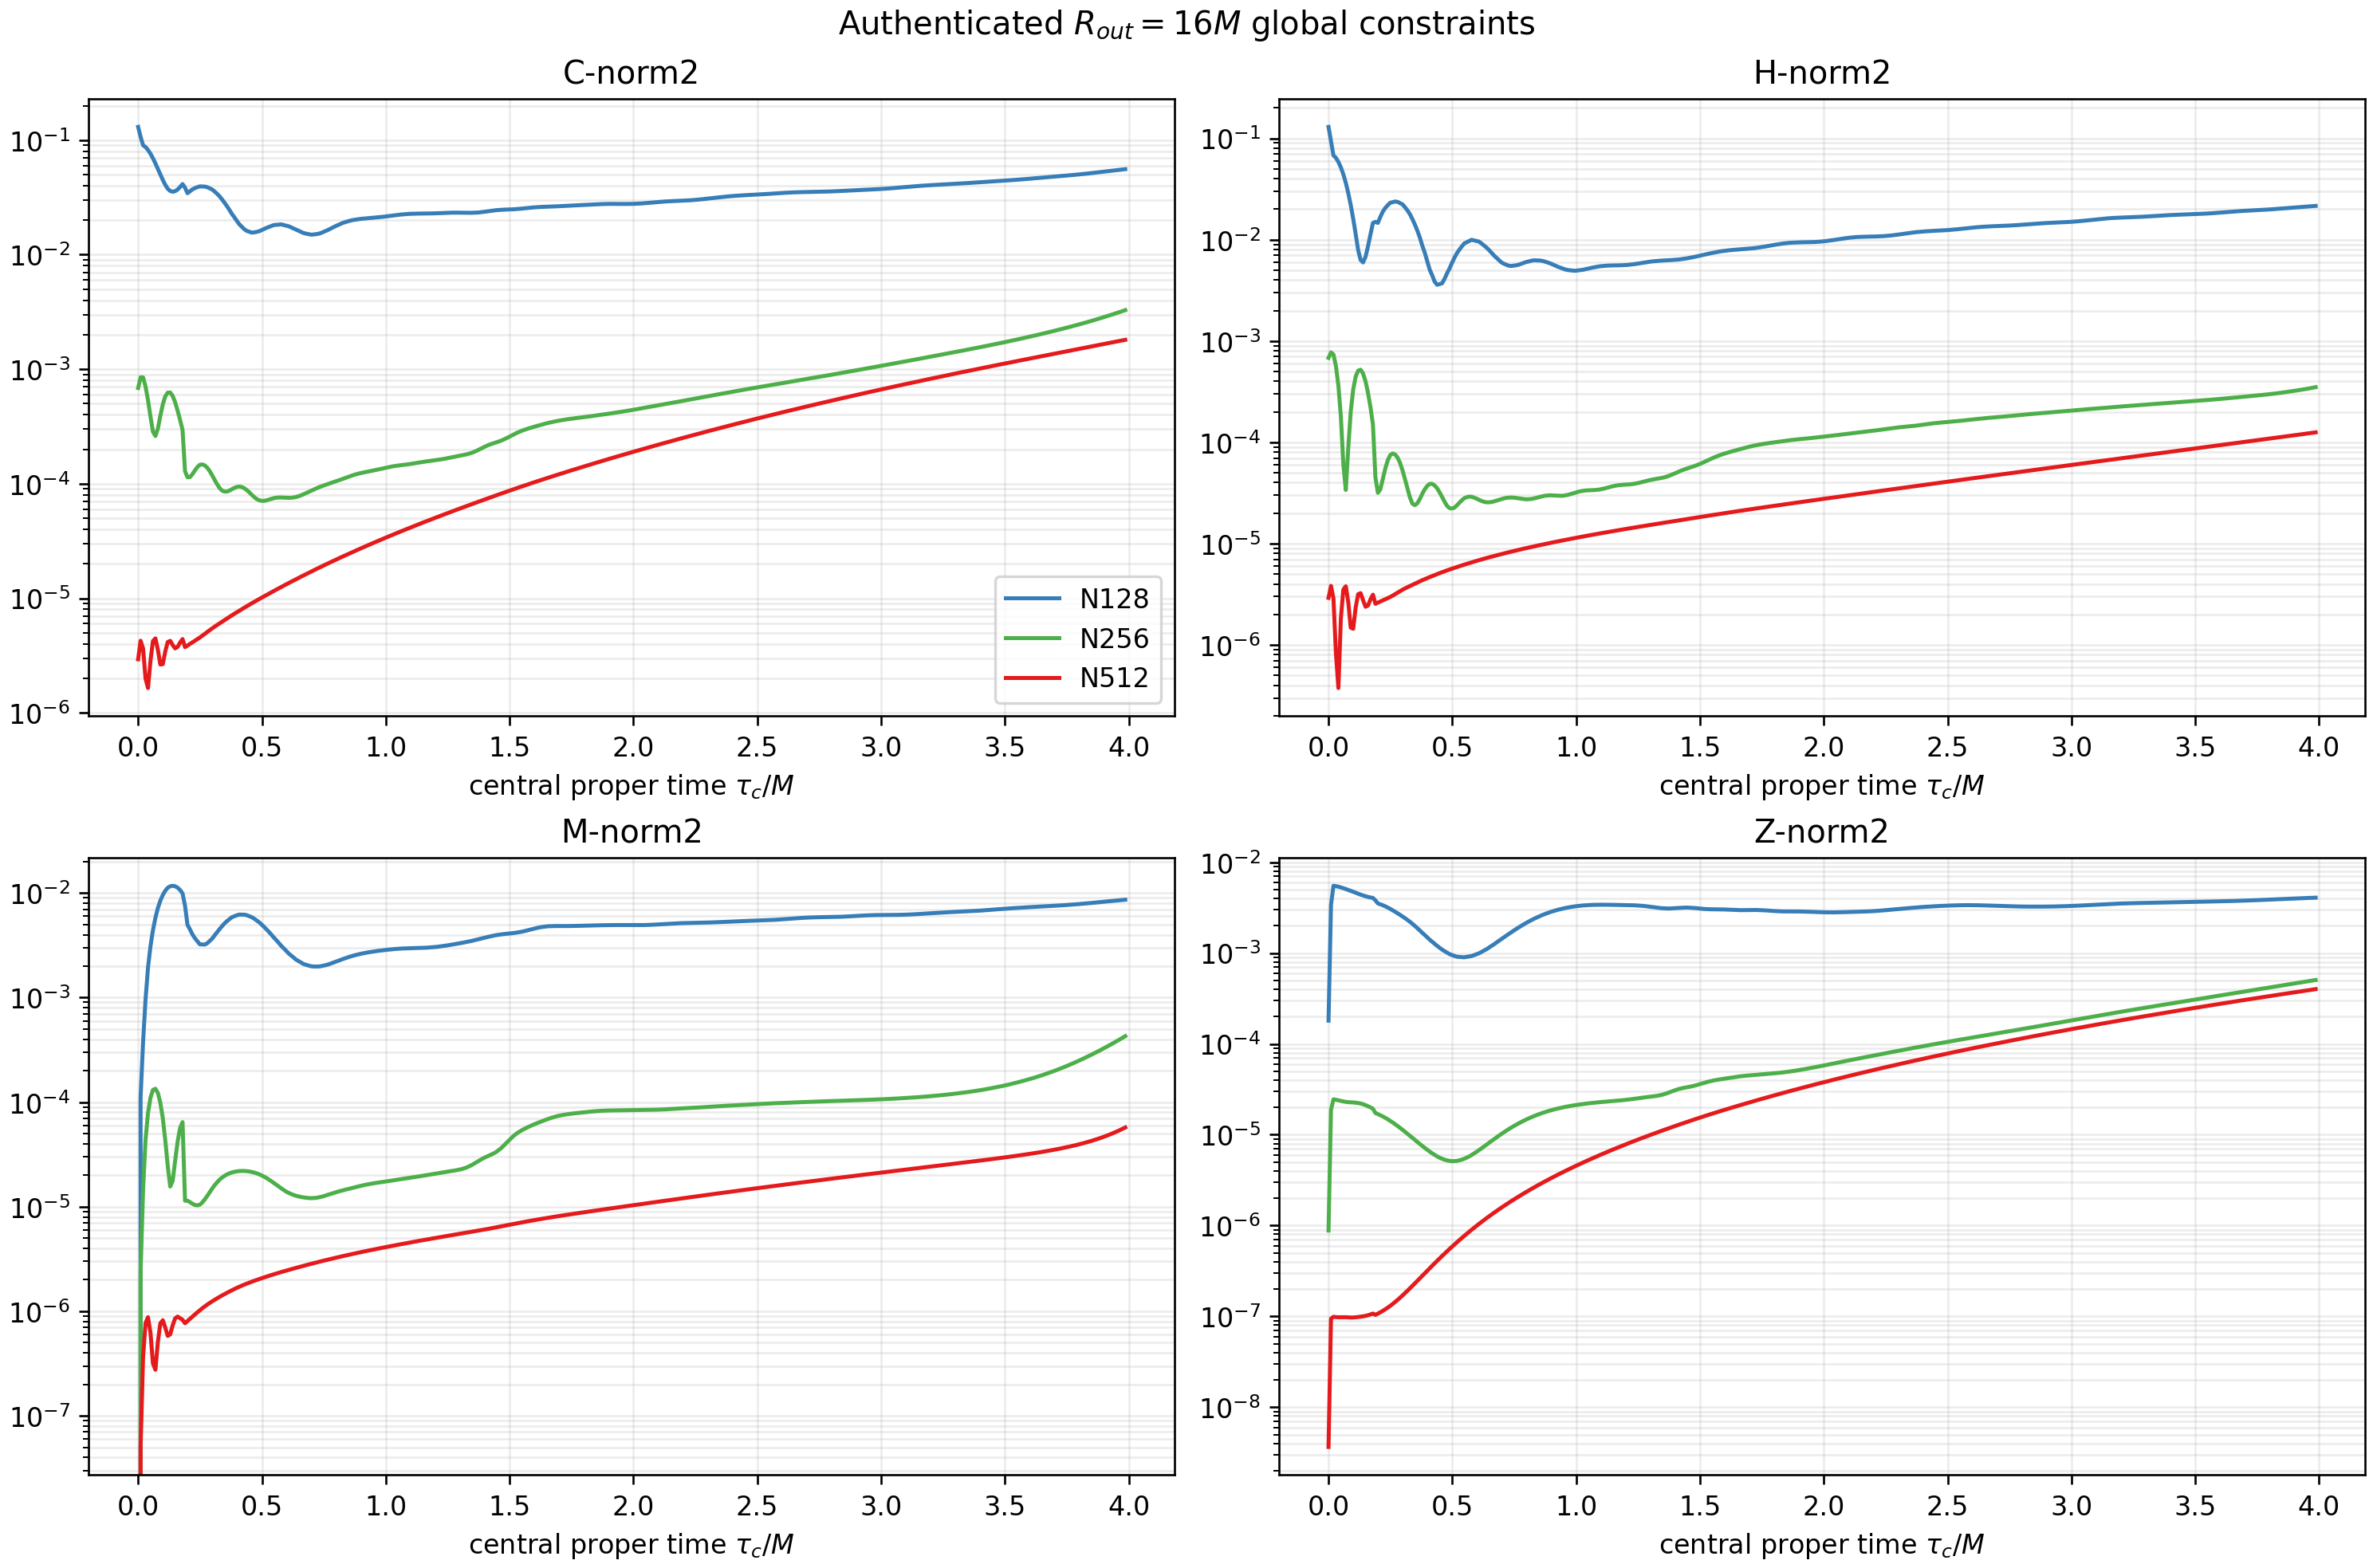
\includegraphics[width=0.97\textwidth]{analysis/figures/original_rout16_global_figure2.png}
\caption{Authenticated $R_{\rm out}=16M$ global constraint histories.}
\end{figure}

\subsection{Large-domain construction and authority}

The new domain is $\rho\in[0,128M]$, $z\in[-128M,128M]$. Three dyadic
minimum levels restore exactly the old inner spacings: 0.25, 0.125, and
0.0625$M$ for N128/N256/N512. The absolute physical ceiling moves from 20 to
23. In the N256 initialization, 33,153 canonical inner vertices have identical
coordinates; 23 of 25 evolved fields agree bitwise and the two Gamma fields
differ by at most $1.94\times10^{-15}$.

The N256 authority ends at $t=6.5M$ with 206 leaves. A separate N256 replay is
bitwise identical in all 264 by 71 history values. N128 and N512 replay every
accepted tree exactly. All runs use one A100; N512 peaks at 36,581 MiB HBM.

\subsection{Restored convergence}

The large-domain full inventories at the common terminal time are:

\begin{table}[H]\centering\small
\begin{tabular}{lrrrrr}
\toprule
 & N128 & N256 & N512 & $p_{128,256}$ & $p_{256,512}$\\
\midrule
C & $5.3530{\times}10^{-2}$ & $1.1984{\times}10^{-3}$ & $3.3856{\times}10^{-5}$ & 5.481 & 5.146\\
H & $2.1422{\times}10^{-2}$ & $2.1681{\times}10^{-4}$ & $1.9176{\times}10^{-6}$ & 6.627 & 6.821\\
M & $8.6008{\times}10^{-3}$ & $3.8660{\times}10^{-4}$ & $1.9891{\times}10^{-5}$ & 4.476 & 4.281\\
Z & $3.5586{\times}10^{-3}$ & $3.4538{\times}10^{-5}$ & $4.7437{\times}10^{-7}$ & 6.687 & 6.186\\
\bottomrule
\end{tabular}
\caption{$R_{\rm out}=128M$ full-domain squared-constraint inventories.}
\end{table}

The N512 old/new full-domain ratios are 53.35, 65.45, 2.88, and 844.68 for
C/H/M/Z. Conversely, $r\le4M$ agrees to about one part in $10^9$. The maximum
small/large difference in $\log_{10}|I(0)|$ is only
$6.7\times10^{-9}$ dex.

\begin{figure}[H]\centering
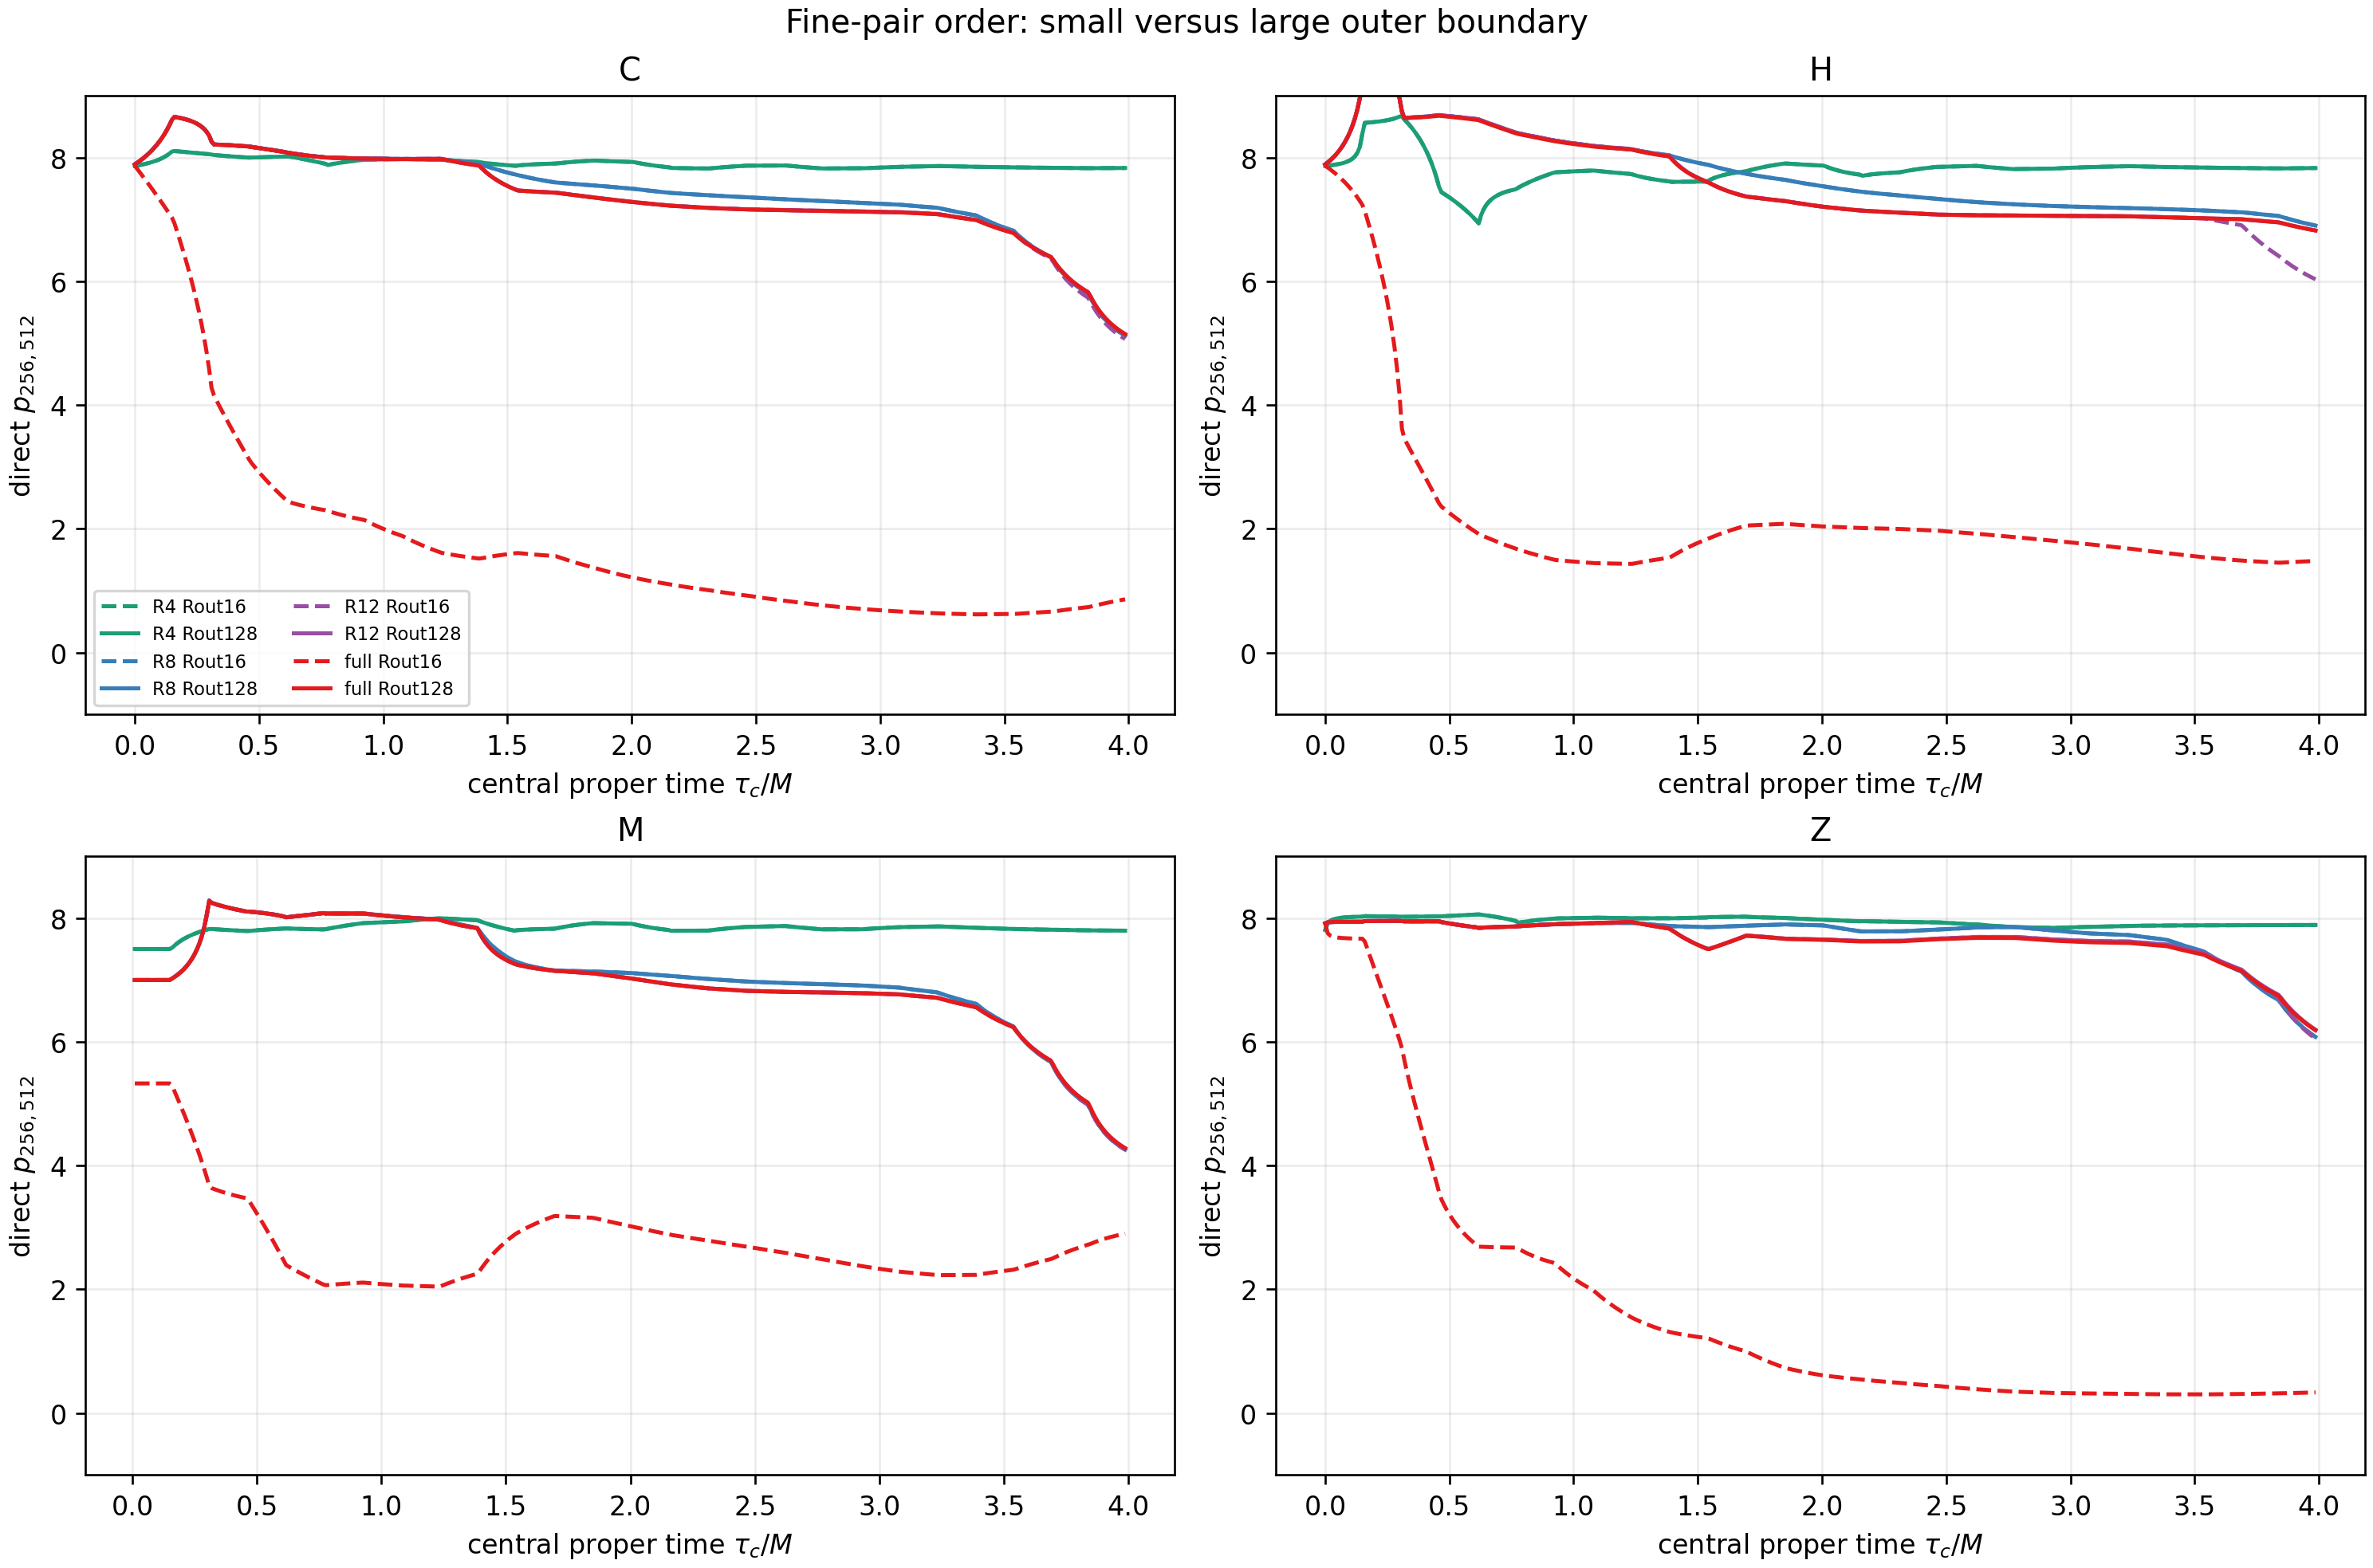
\includegraphics[width=0.98\textwidth]{analysis/boundary_comparison/figures/boundary_fine_pair_orders.png}
\caption{Direct fine-pair order before and after moving the outer boundary.}
\end{figure}

\begin{figure}[H]\centering
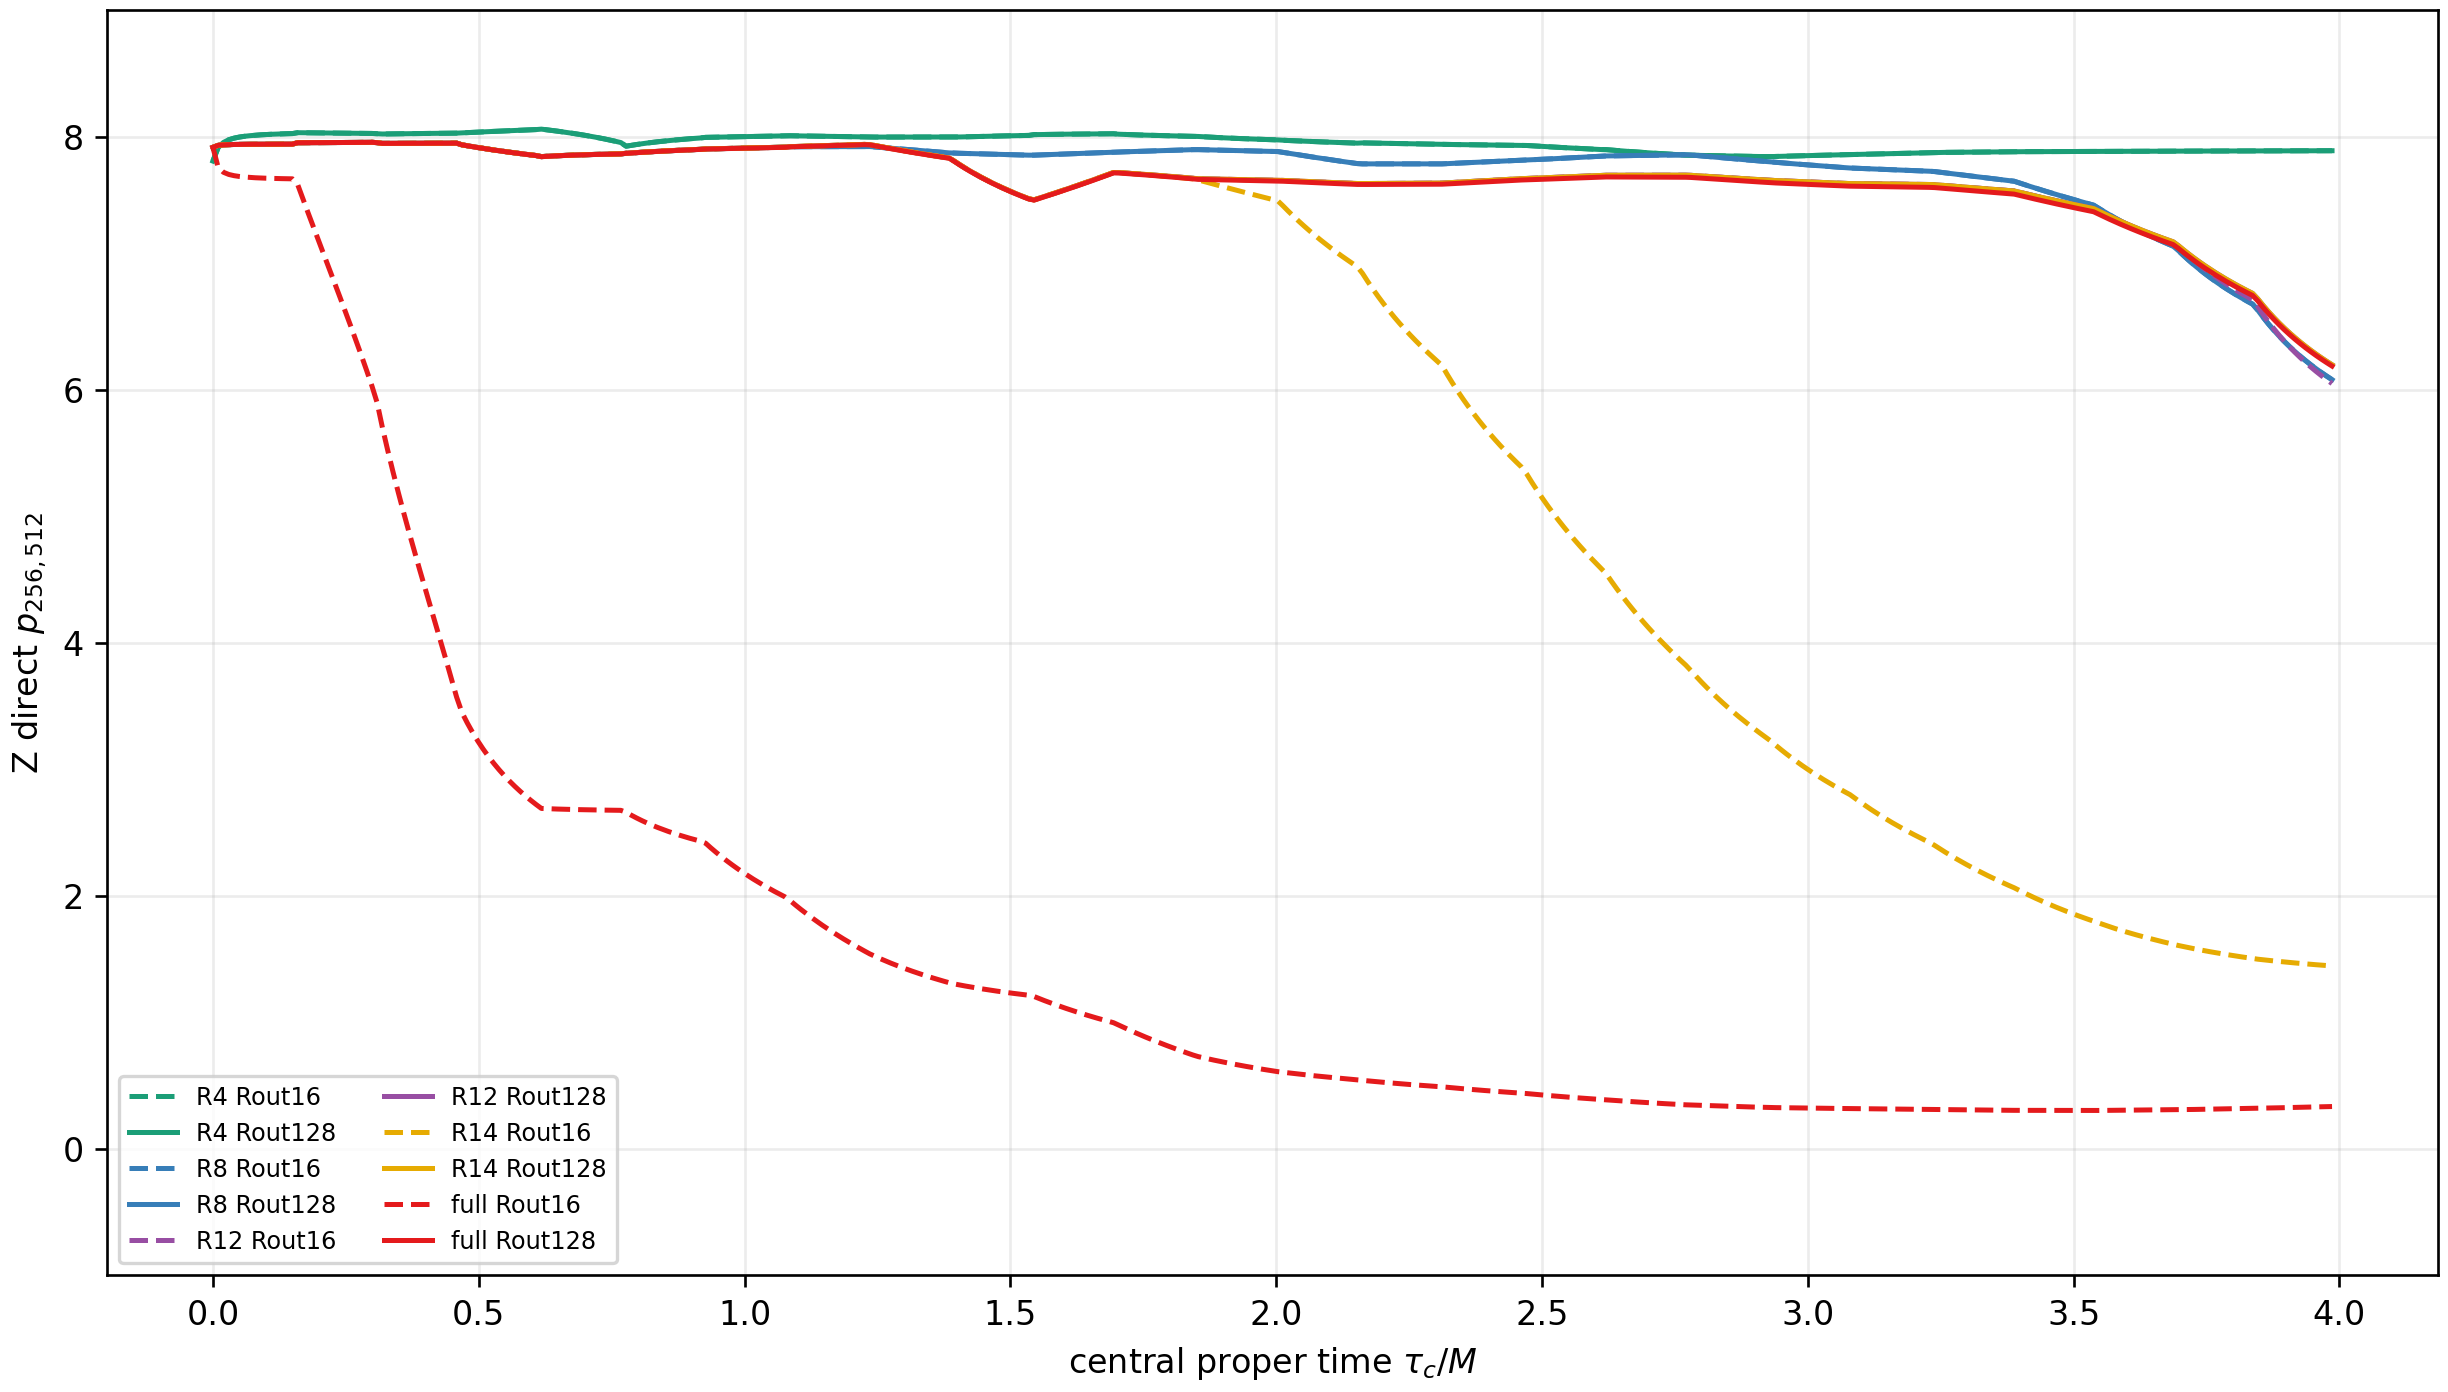
\includegraphics[width=0.88\textwidth]{analysis/boundary_comparison/figures/z_boundary_contamination.png}
\caption{Z convergence identifies the old outer-shell contamination.}
\end{figure}

\paragraph{Boundary verdict.}
\verdict{BOUNDARY\_CONTAMINATION\_CONFIRMED}

\section{Part II: independent N256 KO scan}

Each $R_{\rm out}=16M$ case starts from scratch in native-AMR record mode.
Only KO dissipation changes.

\begin{table}[H]\centering\small
\begin{tabular}{rrrrrrl}
\toprule
diss & C(6.5) & C(9.2) & first late refine & max leaves & terminal $t$ & status\\
\midrule
0.02 & $3.285{\times}10^{-3}$ & 1.032 & 10.2758 & 1526 & 11.191917 & timestep collapse\\
0.05 & $2.693{\times}10^{-3}$ & 0.692 & 10.3658 & 65 & 11.3 & reached tlim\\
0.10 & $2.224{\times}10^{-3}$ & 0.390 & 10.7394 & 86 & 11.3 & reached tlim\\
0.20 & $1.850{\times}10^{-3}$ & 0.168 & 11.1045 & 50 & 11.3 & reached tlim\\
0.50 & $1.518{\times}10^{-3}$ & 0.0437 & none & 50 & 11.3 & reached tlim\\
\bottomrule
\end{tabular}
\caption{Independent N256 KO scan.}
\end{table}

The baseline reaches $dt=7.98\times10^{-9}M$, C=$1.61\times10^{16}$, physical
level 20, and 1,526 leaves before bounded termination. Diss=0.50 has no new
late accepted refinement and ends with C=0.2695. The maximum baseline-relative
central-trace deviation is 0.028, 0.056, 0.086, and 0.110 dex for diss
0.05--0.50 respectively.

\begin{figure}[H]\centering

\includegraphics[width=0.98\textwidth]{analysis/ko_stageC/figures/ko_global_constraints.png}
\caption{Global constraint inventories versus central proper time.}
\end{figure}

\begin{figure}[H]\centering

\includegraphics[width=0.98\textwidth]{analysis/ko_stageC/figures/ko_axisKret_figure3_overlay.png}
\caption{Central curvature trace and authenticated Figure-3 curves, without shifts or rescaling.}
\end{figure}

\paragraph{KO verdict.}
\verdict{KO\_STRONG\_EFFECT}

The late cascade contains a strongly under-damped numerical component.
The evidence does not justify \texttt{KO\_OVERDAMPED}: even diss=0.50 does not
materially displace the central trace over the matched interval. It also does
not justify a production default from one resolution.

\section{Synthesis and next campaign}

The Figure-2 flattening is primarily an outer-boundary effect. The separate
late N256 cascade is strongly sensitive to KO dissipation and therefore is not
a KO-insensitive formulation failure.

The best conservative next configuration is the $R_{\rm out}=128M$ SMR
common-tree workflow with zero Z4 damping and diss=0.20, retaining diss=0.50
as a stability control. A three-resolution extension must show whether the
remaining diss=0.20 growth converges away and whether the small diss=0.50
central-trace difference shrinks. No production numerical parameter is changed
by this report.

\section{Limitations}

The boundary qualification ends at $t=6.5M$; the optional late large-boundary
N256 control was not run. The KO study is one-resolution evidence. No
late-time Figure-3 convergence, horizon, critical exponent, or continuum
stability claim is made. Multi-gigabyte state/restart files remain at the exact
Perlmutter paths recorded in the evidence manifest.

\end{document}

